\section{Plateforme SoC}
Cette partie présente le positionnement de l'IP sur la plateforme SoC.
L'objectif est de mettre l'accent sur les ressources mises en jeu.
Il n'est pour autant pas question d'aller jusqu'à lister le nombre de LUT ou bloc de BRAM.
On choisit de conserver une vue globale.
La carte FPGA retenue pour ce travail fait partie de la famille des Zynq7000 de Xilinx.
Elle intègre deux cœurs de processeur ARM efficacement connectées à de la logique programmable tel qu'on la retrouve dans les FPGA.
Cet assemblage permet de profiter à la fois de la flexibilité qu'apporte le logiciel tout en gardant la possibilité de paralléliser et customiser un circuit numérique.
Ces deux propriétés sont particulièrement intéressantes et permettent d'implémenter des accélérateurs matériels pour le logiciel en profitant d'une communication efficace permise par l'interconnexion AMBA\mbox{\textregistered }.

Implémenter un contrôleur d'interruption sur la plateforme est toutefois un peu particulier.
Cela permet effectivement d'obtenir un traitement des priorités avec une latence réduite et inférieure au cycle horloge.
Mais, la plateforme Zynq-7000 intègre une fonction appelée Generic Interrupt Controller (GIC) qui couvre largement les fonctionnalités de notre IP et même bien d'avantage.
Notre souhait d'intégrer un second contrôleur d'interruption, est a priori difficile à justifier dans un cadre industriel.
Nous ferons l'hypothèse par la suite, pour des raisons pédagogiques, que notre IP a bien ça place et apporte un réel avantage.
Sans se perdre dans les détails techniques, nous essayeront de confirmer que ces deux blocs peuvent cohabiter dans le même SoC sans entrer en conflit.
La figure \ref{fig:soc} illustre le positionnement du contrôleur d'interruption (notre IP) sur la plateforme SoC.
\begin{figure}[H]
    \centering
    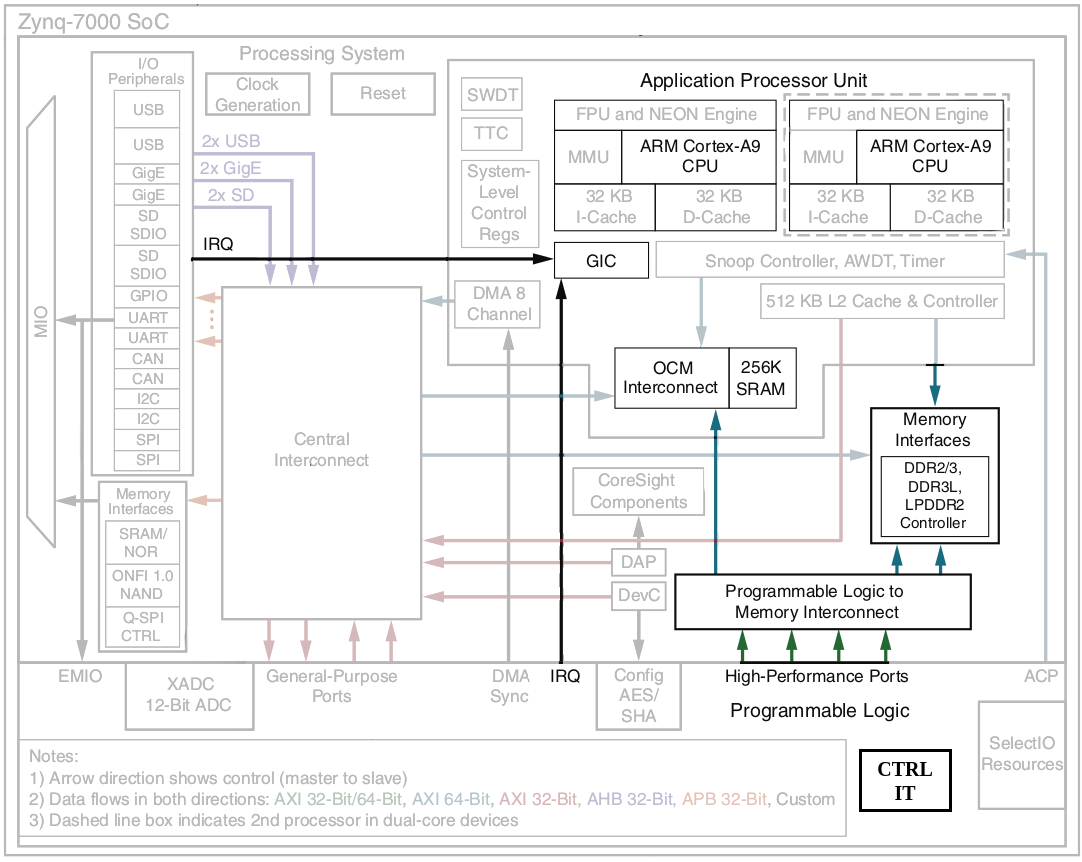
\includegraphics[width=0.72\linewidth]{global_bloc_diagram_zynq.drawio.png}
    \caption{Positionnement de l'IP sur la plateforme SoC.}
    \label{fig:soc}
\end{figure}
Elle se place naturellement en bas à droite dans la partie "programmable logic" (PL).
Son implémentation repose bien sur un ensemble de ressources logiques composé de LUT, bascules, RAM, etc.
La figure \ref{fig:soc} tirée de la documentation Xilinx \cite{Tech_Man_Xilinx} a été modifiée afin de mettre en avant les éléments en lien avec notre IP.
Elle n'a pas vocation à être parfaitement exhaustive.
On retrouve parmi les fonctions clés le "Programmable Logic To Memory Interconnect".
Il est composé de ports AXI hautes performances fournissant un accès depuis la PL à la DDR et à la mémoire de la puce\footnote{Dans la documentation Xilinx on retrouve le terme on-chip memory (OCM)}.
Ses quatre ports AXI allant de la PL aux CPUs (Processing System PS) sont configurables en tant qu'interfaces 32 bits ou 64 bits.
C'est par cette interface que les échanges entre notre IP et le processeur auront lieu.

\gap
La particularité du contrôleur d'interruption est d'avoir une seconde interface de communication avec les autres IPs.
Cette dernière est formée de l'ensemble des signaux \texttt{nIT\_xxx} indicateurs d'une requête d'interruption.
Le terme "les autres IP" fait référence aux IPs "sur mesure" implémentées dans la PL et celle déjà présente dans l'"I/O peripherals" comme le SPI, l'UART, etc.
Il y a donc deux sources bien distinctes.
Nous pensons, en nous basant sur la documentation \cite{Tech_Man_Xilinx}, qu'il est possible de rediriger toutes les sources d'interruptions vers notre IP.
La figure \ref{fig:GIC} illustre le chemin des signaux \texttt{nIT\_xxx} et \texttt{nIT\_CPU} en se basant sur l'architecture du GIC.
\begin{figure}[H]
    \centering
    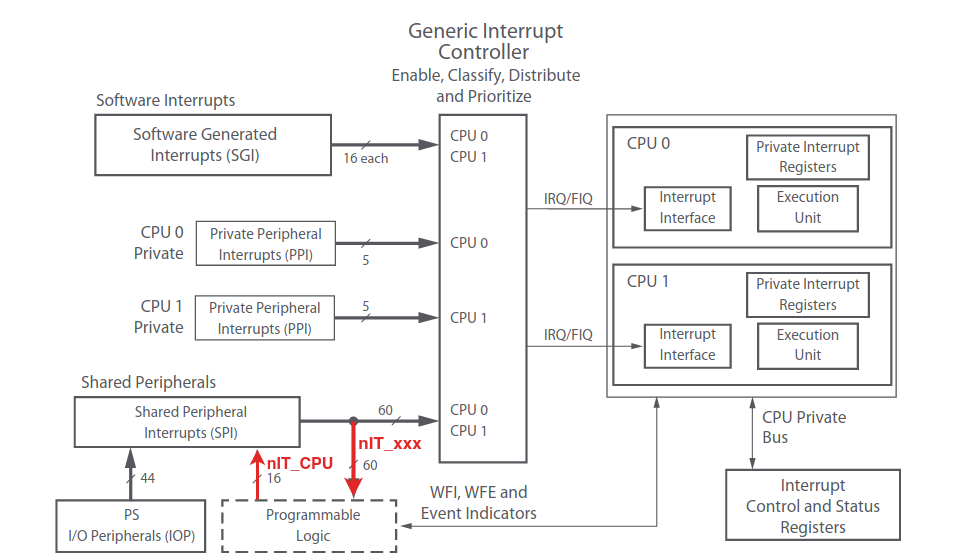
\includegraphics[width=0.8\linewidth]{GIC.drawio.png}
    \caption{Chemin des sources d'interruptions d'après l'architecture du GIC.}
    \label{fig:GIC}
\end{figure}
La solution que nous proposant est de récupérer les requêtes des "I/O peripherals" via le bus marqué \texttt{nIT\_xxx}.
Les sources émises par les IP "sur mesure" peuvent être connectée directement à notre IP sans passer par le GIC.
Le signal \texttt{nIT\_CPU} peut lui être transmis via parmi les 16 sources provenant de la PL.
Il faudra au préalable masquer dans le GIC les sources provenant des "I/O peripherals" sans quoi elles seraient traitées deux fois.

\gap
Le dernier élément mis en évidence par la figure \ref{fig:soc} est naturellement l'unité processeur applicatif.
L'aspect multicœur est complexe.
Il est difficile de se projeter sur la gestion des interruptions par ces deux processeurs ARM A9.
Cela dépend aussi de la stratégie de l'application.
Nous ferrons l'hypothèse que les interruptions sont traitées de la même manière que sur une architecture monocœur.
À la réception du signal \texttt{nIT\_CPU}, l'adresse de branchement est lue, la routine est exécutée et le flag du périphérique est remis à zéro.
Le cœur utilisé est indifférent de ce point de vue.
